\chapter{Propulsion system}
\section{Engine cycle}
\qquad The spacecraft uses electrically-driven turbo pumps to feed the oxidizer as well as the fuel to the engine. The propellant and oxidizer are each driven out of their tanks at low pressure, where after a turbo pump in each propellant line strain raises their pressures. As the oxidizer strain has a higher mass flow rate and faces a large pressure drop in the catalyzer, the respective pump is also more powerful as a result. The turbo pumps are driven electrically by electric motors which use large batteries for their power intake. These batteries offer enough charge for one maximum burn time of 900 seconds, after which they are re-powered by a fuel cell which runs on hydrogen and the hydrogen peroxide decomposition product oxygen. This will be explained further in \autoref{sec:10-3}. In order to demonstrate how exactly the engine cycle is made up, a flow schematic is shown in the following. Firstly, the pressurization system is shown in \autoref{fig1}.
\begin{figure}[H]
	\centering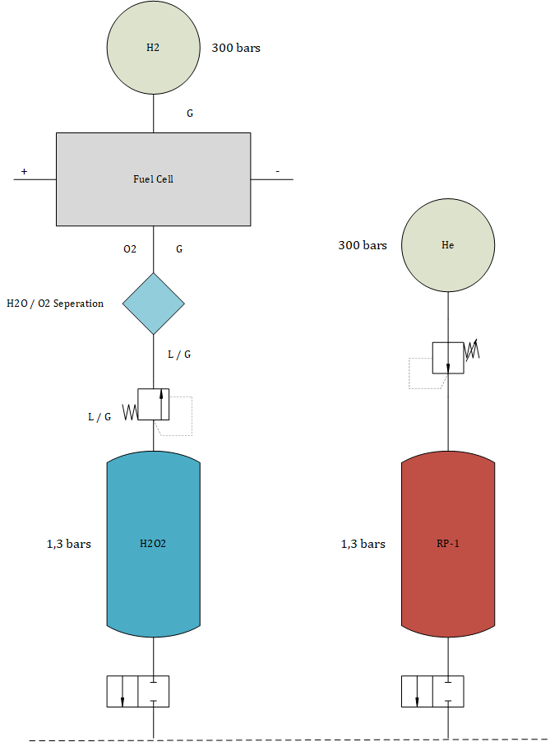
\includegraphics[width=0.5\linewidth]{pressurizationsystem}
	\caption{Flow Schematic - Pressurization system}\label{fig1}
\end{figure}

As the figure shows, only the RP-1 tank is pressurized by pressurization gas, using a $300$ bars helium tank. The hydrogen peroxide has certain decomposition characteristics which enable it to self-pressurize due to the rising pressure upon vaporization. The critical point of hydrogen peroxide is at around $150$ degrees Celsius and $1.5$ bars, meaning that if the thermal control is sufficiently reliable, a tank pressure of around $1.3$ bars can be maintained by self-pressurization. The control system and more details will be explained in \autoref{sec:10-3}. The $300$ bars H2 Tank that can be seen in the pressurization system flow schematic is therefore not a pressurization tank, but a tank for the sole purpose of running the fuel cell in combination with the oxygen which is separated from water, which is the second decomposition product of hydrogen peroxide. The separation works by simply condensing the water and allowing the gaseous oxygen to pass through a filter. Both the RP-1 tank and the H2O2 tank have a main valve after their outlets, which are visible in \autoref{fig1}. The remaining feeding system is shown in the second part of the flow schematic, depicted in \autoref{fig2}.

\begin{figure}[H]
	\centering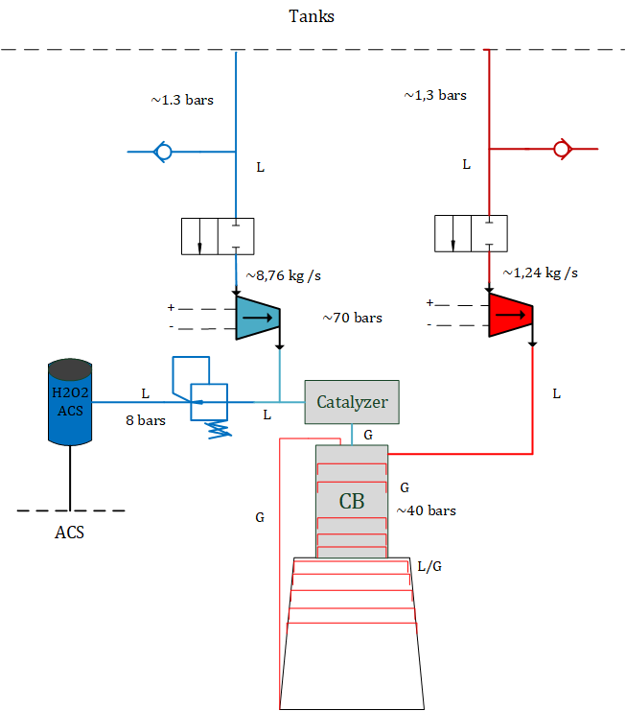
\includegraphics[width=0.7\linewidth]{flowenginesection}
	\caption{Flow Schematic - Engine section}\label{fig2}
\end{figure}
The fueling ports for RP-1 as well as hydrogen peroxide extend to the left- and right-hand-side of the top of the figure. Check valves are situated at these points to only allow propellant flowing in. A second main valve for both propellants is installed just before the turbopumps, which are closed during refueling. While the RP-1 is then funneled through cooling channels in the regenerative cooling system, the oxidizer runs into a catalyzer, where a rapid decomposition reaction splits the hydrogen peroxide into its reactive products for combustion. A second oxidizer strain is guided towards a pressure regulation valve, behind which it continues into a buffer tank of hydrogen peroxide for monopropellant use in the ACS. The catalyzers for ACS thrusters are located in close proximity to their respective combustion chambers. The ACS is not depicted as a flow schematic.

\section{RCS / ACS}

In the previous section we mention that we are going to use hydrogen peroxide as a monopropellant for our Reaction Control System. Indeed, hydrogen peroxide can be used as a quite good RCS propellant. \\

At the moment, the biggest part of the monopropellant thruster using $H_2O_2$ are test bench engine. This is because of the difficulty to characterize the engine and its parameters. \\

Hydrogen peroxide is usable as a monopropellant because of its natural decomposition. As we are going to see on the Catalyzer part further on the report $H_2O_2$ can be decomposed in $H_2$ and $H_2O$. That's this decomposition we are going to use inside our thruster. \\
When hydrogen peroxide goes through a catalyser it decomposes and generates a great amount of heat, up to $1000K$. This two factors create steam at a very high temperature and pressure; it's this steam that creates our thrust.\\

Before designing the engine and its characteristics we need to choose the positioning of the thrusters. In order to do that, we based our design on the American Space Shuttle which use cluster of small thrusters all around the spacecraft to allow a good maneuverability.  

\begin{figure}[H]
    \centering
    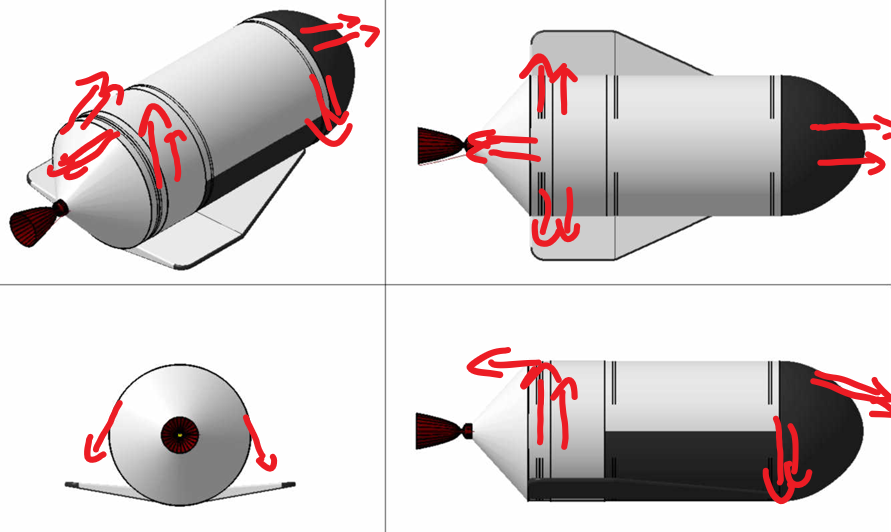
\includegraphics[width=\linewidth]{shiprcs}
    \caption{RCS thruster repartition}
\end{figure}

We are going to use 6 different clusters spread over the craft, each cluster is composed of 2 thrusters for a total of 12. This disposition allow to manipulate every axis. \\

Now we need to compute the characteristic of the thruster, to do so we used RPA (a NASA software to compute the parameters of a thruster based on the propellant and several other characteristics) and some papers of recent studies about hydrogen peroxide thruster. \\

We assumed a chamber pressure of $10bars$ and a thrust of $100N$, then we use RPA to get the other parameters.

\begin{itemize}
    \item Combustion temperature: $1223K$
    \vspace{-0.4cm}
    \item Ejection temperature: $424K$
    \vspace{-0.4cm}
    \item Ejection pressure : $0.094bars$
    \vspace{-0.4cm}
    \item $\gamma = 1.335$
    \vspace{-0.4cm}
    \item $R = 368.6$
    \vspace{-0.4cm}
    \item $ISP = 140s$
\end{itemize}

With these parameters we can then compute every other parameters we want for the thruster and especially the mass flow rate which is necessary to have a correct mass budget. 

$$c^* = \sqrt{\frac{R T_c}{\gamma}}\times \frac{\gamma + 1}{2}^{\frac{\gamma + 1}{2(\gamma - 1)}}$$

Throat characteristics:
$$T_t = T_c \left(\frac{2}{\gamma + 1}\right) \hspace{20pt}
P_t = P_c \left(\frac{2}{\gamma + 1}\right)^{\frac{\gamma}{\gamma - 1}} \hspace{20pt}
\rho = \frac{P_t}{R T_t} \hspace{20pt}   u_t = \sqrt{\gamma R T_t}$$

Exhaust characteristics:
$$M_e = \sqrt{\frac{2}{\gamma - 1}\left[\left(\frac{P_c}{P_e}\right)^\frac{\gamma - 1 }{\gamma} - 1 \right]} \hspace{20pt} T_e = \frac{T_c}{1 + \frac{\gamma - 1}{2}M_e^2}  \hspace{20pt} \rho_e = \frac{P_e}{R T_e}$$

\clearpage

Thus we can compute the area ratio and the thrust coefficient:

$$\frac{A_e}{A_t}= \frac{1}{M_e}\left[\frac{2}{\gamma + 1}\left(1 + \frac{\gamma - 1}{2} M_e^2 \right)\right]^{\frac{\gamma + 1}{2(\gamma - 1)}}$$

$$ C_F = \gamma \sqrt{\left(\frac{2}{\gamma + 1}\right)^{\frac{\gamma + 1}{\gamma - 1}}\frac{2}{\gamma - 1} \left[ 1 - \left(\frac{P_e}{P_c}\right)^{\frac{\gamma - 1}{\gamma}}\right]} + \frac{P_e - P_a}{P_c}\frac{A_e}{A_t} $$ 

\vspace{1cm}

Finally we can compute the exhaust velocity, throat area and the mass flow: 

$$c = C_F c^* \hspace{20pt} A_t = \frac{F}{C_F P_c} \hspace{20pt} \dot m = \frac{P_c A_t}{c^*}$$

From our assumptions and the results of RPA we finally have:

\begin{itemize}
    \item Exhaust velocity: $c=617.38m/s$
    \vspace{-0.4cm}
    \item Mass flow rate: $\dot m = 0.105 kg/s$
\end{itemize}

The most important value for us is the mass flow rate as it allows us to compute the propellant mas needed to perform our maneuvers. \\

In addition of the thrusters we also need another system which is the Reaction Wheels. This systems which is separated in 3 different wheel, one for each axis, and allow to rotate the entire craft on the 3 axis with the the reaction motion applied by the rotation of the wheel.
\clearpage

\section{Multi-usage of hydrogen peroxide}
\label{sec:10-3}

\section{Propellant tanks}

\section{Catalyzer}
Besides the advantages of $H_2O_2$ there is one major drawback that we have to take into account. This drawback is that $H_2O_2$ needs to be decomposed in $H_2$ and $H_2O$ in order to react with RP-1. 

\begin{figure}[H]
	\centering
	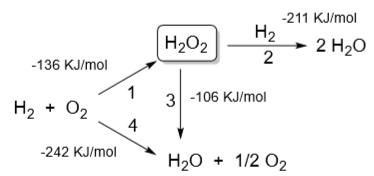
\includegraphics{H2O2}
	\caption{$H_2O_2$ chemical decomposition process}
\end{figure}

This decomposition is natural but at a low rate whereas we need a very high decomposition rate in order to feed the combustion chamber and sustain a proper flame. This decomposition is an exothermic decomposition. That's why we need a catalyser. \\

This catalyser needs to be placed between the turbo pump and the injectors. It allows to decompose the $H_2O_2$ at the last time. \\

The way a catalyser works is pretty simple; the $H_2O_2$ goes through a catalyst bed of silver pellets, reacts and generates heat. 
Why silver ? We chose silver because is the mostly used catalyser for $H_2O_2$. However, a lot of other different material exists, like Platinum, Manganese or even Gold but these materials are rarely used due to their cost and also the fact that they need to be made in complex alloy in order to optimize the reaction. 

\begin{figure}[H]
	\centering
	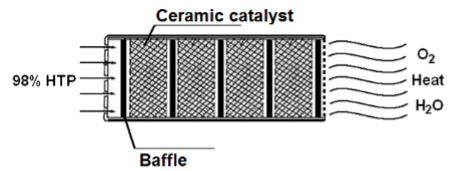
\includegraphics{catalyst}
	\caption{Example of catalyst bed}
\end{figure}

The figure above shows basically how a catalyser works. To have an idea of the shape of ours we just have to swap the ceramic catalyst by silver catalyst. So, it will be a steel cylinder filled with small spherical silver pellet separated by some baffles (silver grid mesh). \\

An important characteristic of the catalyser is the pressure drop it creates. This pressure drop influences the whole feeding system, the turbo pump sizing and even the injector design. that's why we need to characterize the pressure drop created by the catalyser. In order to do so, we are going to use the Ergun equation for packed bed reactor:

$$
\frac{\Delta p}{L} = 151.2 \frac{\mu}{d^2}\frac{(1-\epsilon)^2}{\epsilon^2}u + 1.8 \frac{\rho}{d}\frac{1- \epsilon}{\epsilon^3}u^2
$$

With $\mu$ the dynamic viscosity, $\epsilon$ the porosity, $d$ the pellet diameter, $\rho$ the density, $L$ the length of the bed and $u$ the velocity. \\

In this equation we need some important component such as $\epsilon$. The porosity is complicated to compute and need to be model. According to a recent research we determined a porosity of $0.3802$ with a pellet diameter of 5mm.

\begin{figure}[H]
	\centering
	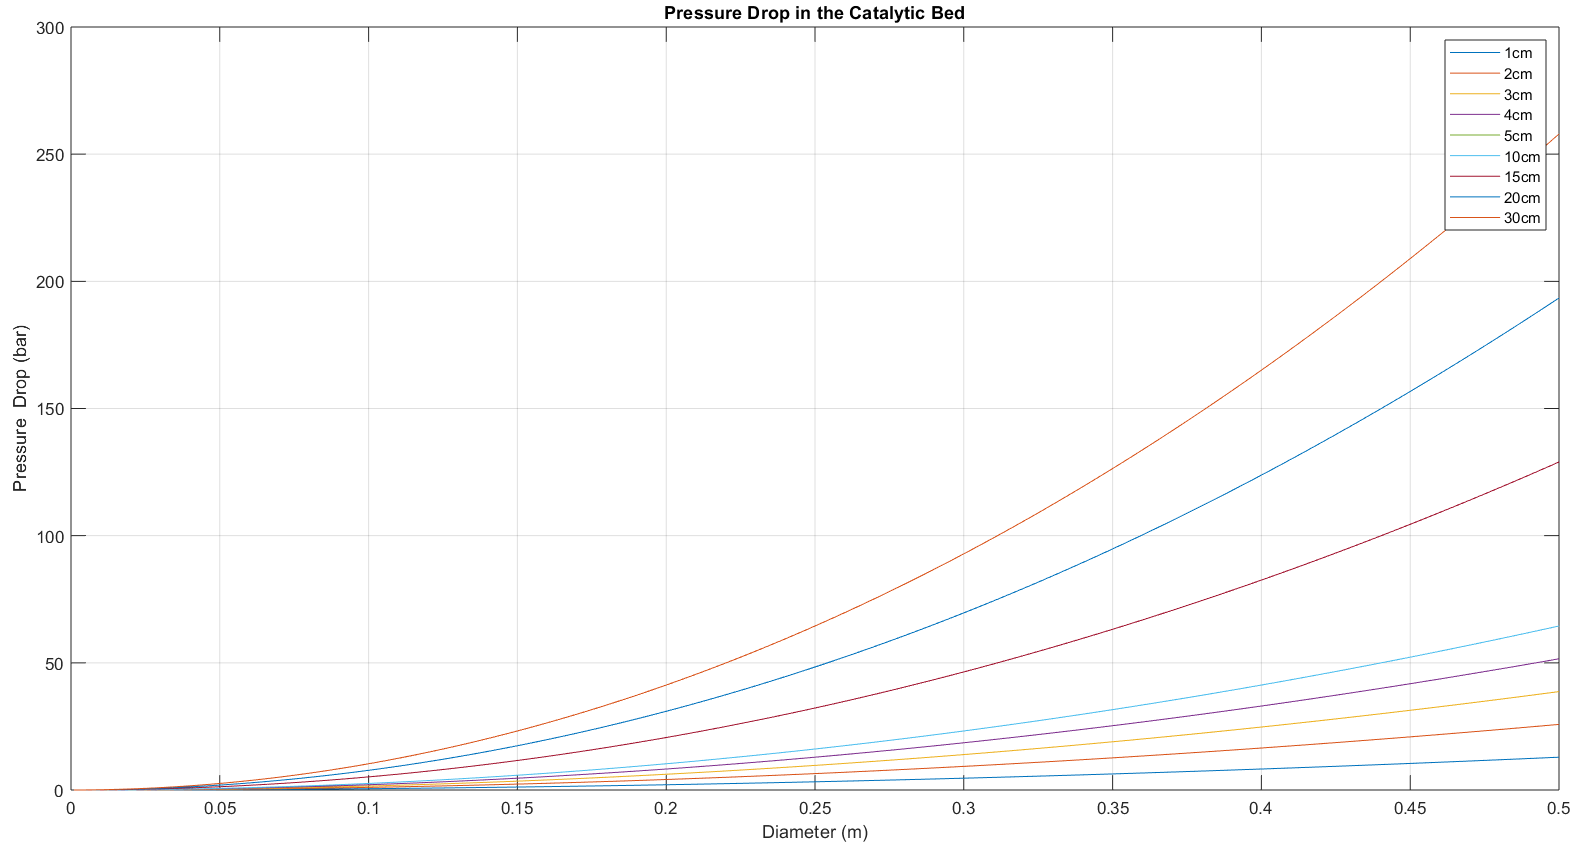
\includegraphics[width=\linewidth]{pressuredrop}
	\caption{Pressure drop depending on the size of the catalyst bed}
\end{figure}

We see on the graph that the pressure drop rise quickly with the size of the bed. So we need to limit the size of our catalyser in order to not oversize the turbo pump. To do so, we chose to limit our pressure drop to around 30 bars. Finally we obtain a cylinder of 20 cm of diameter and 20 cm of length. \\

This geometry allows the catalyser to provide a sufficient decomposition rate, a "contained" pressure drop and size. It also generates a great heat as high as $1000K$ at the exit of the catalyst bed. 

\section{Injectors}

To design our injectors we made some research and went through the literature about injector for hypergolic injector. We found interesting results in this paper\footnote{The design and main performance of a hydrogen peroxide/kerosene coaxial-swirl injector in a lab-scale rocket engine (2017)}. Their goal was to design a small attitude control system hydrogen peroxide/RP-1 thruster, to do so they compared different kind of injectors.


\begin{figure}[H]
    \centering
    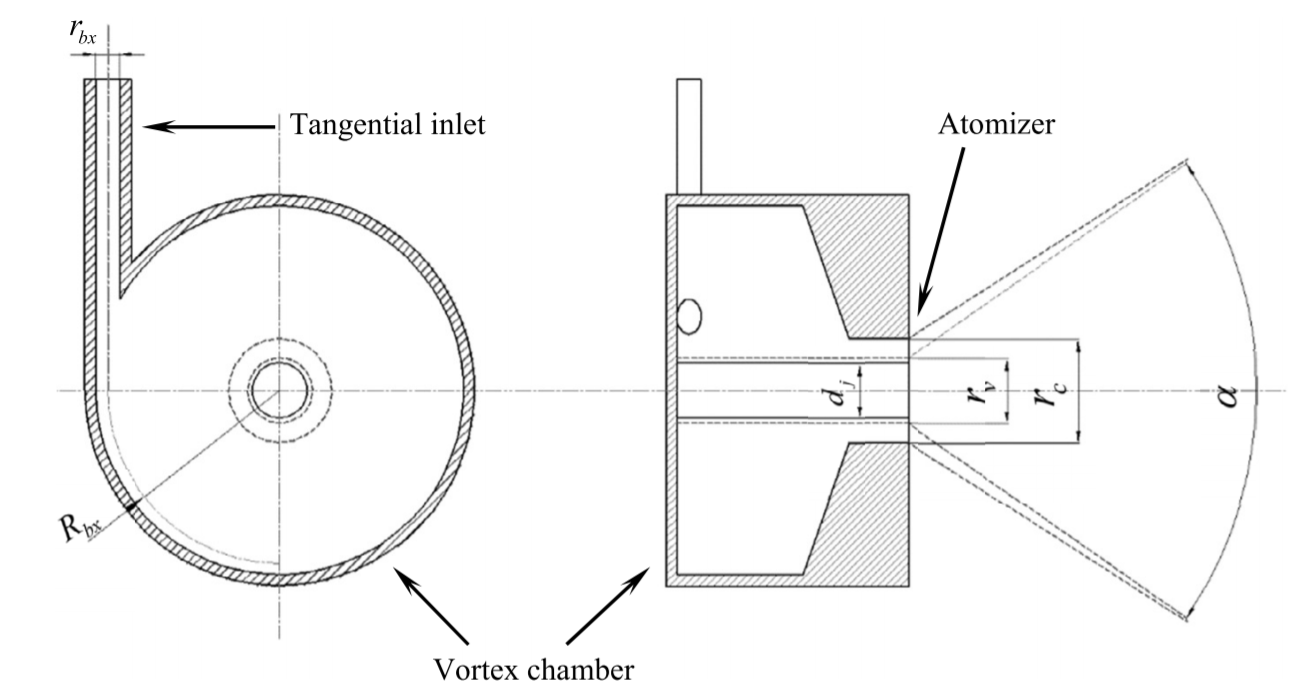
\includegraphics[width=\linewidth]{swirl}
    \caption{Cross section of a swirl injector}
\end{figure}

\section{Feeding system}
After having designed most of our propulsion system. We need to carefully link them by designing our feeding system. The biggest challenge is to create a system that will both fit in our spacecraft and deliver the right amount of propellant from the tanks to the engine through our different, required other subsystems.\\

The general pressure loss in a system is given by :

$$
\Delta P = K\frac \rho 2 w^2
$$

With $K$ depending on the type of change in system geometry as follow : 
\begin{figure}[H]
	\centering
	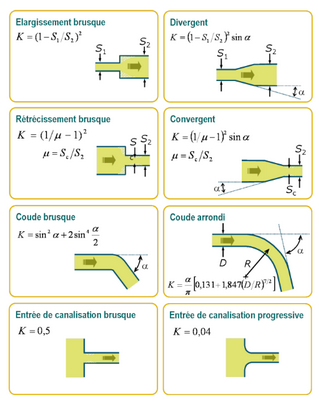
\includegraphics[height=12cm]{pertecharge}
	\caption{$K$ values for geometry changes}
\end{figure}
In our case, we will use the progressive line entering loss $K = 0.04$ and the bends $ K(\alpha) = \sin^2(\alpha) + 2\sin^4\bigg(\frac\alpha 2\bigg)$. Another $K$ will also be used for the entrance of the injector, which will be specified later on.\\

For manufacturing costs and simplicity purposes, we choose to only use $45^\circ$ bends which will result in $K_{bends}=0.5429$.\\

With that and the length measurements in mind, we designed the following feeding system layout for which we will then calculate the pressure variations along it :
\begin{figure}[H]
	\centering
	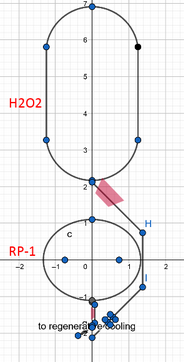
\includegraphics[height=10cm]{feeding}
	\caption{Feeding system layout (To scale)}
\end{figure}
\begin{figure}[H]
	\centering
	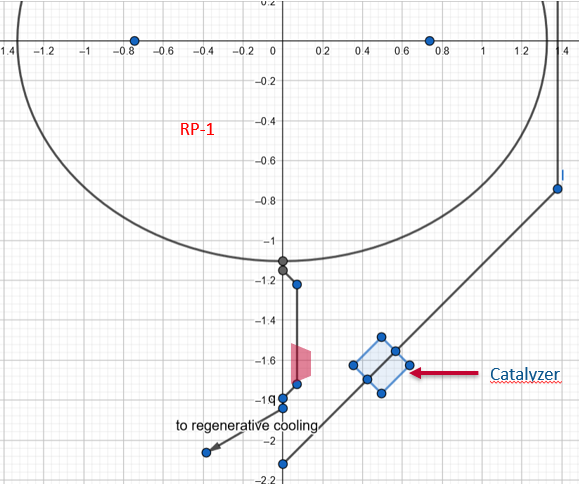
\includegraphics[height=8cm]{feedingzoom}
	\caption{Feeding system layout - Zoomed (To scale)}
\end{figure}
\subsection{Line diameters}
In order to choose our line diameters, we can first use our volume flow and then get the line area from it and then at the end, the line diameter.\\
\underline{Fuel} 
\begin{align}
\dot{V_f}&= \frac{\dot{m_f}}{\rho_f} = 0.0015298m^3/s\\
A_{line_f} &= \frac{\dot V_f}{w_f}=5.21\times 10^{-5} mm^2\\
d_{line_f} &= 2\sqrt{\frac{A_{line_f}}{\pi}} = 8.1447mm
\end{align}
As we are trying to insure a high injection velocity and to insure a certain margin in pressure and velocity, we will choose a line diameter of $7$ mm for the fuel feeding system.
\underline{Oxidizer}
\begin{align}
\dot{V_o}&= \frac{\dot{m_o}}{\rho_o} = 0.006042m^3/s\\
A_{line_o} &= \frac{\dot V_o}{w_o}=0.000275 mm^2\\
d_{line_o} &= 2\sqrt{\frac{A_{line_o}}{\pi}} = 18mm
\end{align}
In this case, we will choose a line diameter of $15$ mm for the oxidizer.

\subsection{Fuel feeding system}
The following items in our fuel feeding system will cause pressure drops :
\begin{itemize}
	\item Tank exit : $K=0.04$
	\item 4 $\times$ $45^\circ$ bends : $K = 0.5429$ for each
	\item Straight line losses : $\Delta P = \frac \rho 2 w^2 f \frac{L}{D}$
	\item Friction coefficient : $f = 0.02$
	\item Regenerative cooling : $\Delta P = 0.25$ bar
	\item Fuel injection : $\Delta P = 9.3843$ bars
\end{itemize}

With our current layout, we have $5$ straight lines which will cause pressure losses on the fuel side. Three of them are before the turbopump which is placed at the end of the third straight section, right before the third bend. We consider a velocity of $8$ m/s before the turbopumps and of $v_{inj}=29.363$ m/s after. The line loss for each section is given by : 
$$
\Delta P = \frac {810} 2 w^2 \times 0.02 \times \frac{L_{section}}{0.007}
$$
\begin{enumerate}
	\item First section ($L_{section}=0.05m$) : $\Delta P = 0.037029$ bar
	\item Second section ($L_{section}=0.1m$) : $\Delta P = 0.074057$ bar
	\item Third section ($L_{section}=0.5m$) : $\Delta P = 0.37029$ bar
	\item Fourth section ($L_{section}=0.1m$) : $\Delta P = 0.997699$ bar
	\item Fifth section ($L_{section}=0.05m$) : $\Delta P = 0.49884$ bar
\end{enumerate}
There are also two different values for the bend losses depending on the position of the bend (before or after the turbopump), we have $2$ of each :
\begin{itemize}
	\item $\Delta P_{before} = 0.14072 $ bar
	\item $\Delta P_{after} = 1.8957$ bar
\end{itemize}
The tank exit loss is :
$$
\Delta P_{exit} = K_{exit} \times \frac{\rho_F}2 \times 8 ^ 2 = 0.010368\text{ bar}
$$
\subsection{Oxidizer feeding system}
The following items in our oxidizer feeding system will cause pressure drops :
\begin{itemize}
	\item Tank exit : $K=0.04$
	\item 4 $\times$ $45^\circ$ bends : $K = 0.5429$ for each
	\item Straight line losses : $\Delta P = \frac \rho 2 w^2 f \frac{L}{D}$
	\item Friction coefficient : $f = 0.02$
	\item Catalyzer : $\Delta P = $ bars
	\item Oxidizer injection : $\Delta P = 4.9599$ bars
\end{itemize}

On this part of the feeding system, we also have $5$ sections and $4$ bends of $45^\circ$ each. We also consider a velocity of $8$ m/s before the turbopump and $21.971$ m/s after. However, due to the larger distances (due to our tank layout), the turbopump's position in the feeding system is different and is now positioned after the first bend, right at the beginning of the second straight line. This results in $3$ bends being at high velocity and $1$ at relatively slower velocity.\\

Here, each straight line loss section is given by : 
$$
\Delta P = \frac {1450} 2 w^2 \times 0.02 \times \frac{L_{section}}{0.015}
$$
With : 

\begin{enumerate}
	\item First section ($L_{section}=0.05m$) : $\Delta P = 0.030933$ bar
	\item Second section ($L_{section}=1.95m$) : $\Delta P = 9.0992$ bars
	\item Third section ($L_{section}=1.4836m$) : $\Delta P = 6.9228$ bars
	\item Fourth section ($L_{section}=1.15m$) : $\Delta P = 5.3662$ bars
	\item Fifth section ($L_{section}=0.6m$) : $\Delta P = 2.7997$ bars
\end{enumerate}

For the bends, we have :

\begin{itemize}
	\item $\Delta P_{before} = 0.2519 $ bar ($1$ of them)
	\item $\Delta P_{after} = 1.0614$ bar ($3$ of them)
\end{itemize}

The tank exit loss is :
$$
\Delta P_{exit} = K_{exit} \times \frac{\rho_o}2 \times 8 ^ 2 = 0.01856\text{ bar}
$$
\section{Turbo pumps}
As most of our subsystems have a defined pressure drop due to their specific design, we have made the choice to use this feeding system design with all losses included to then design our turbopumps to have a pressure rise in accordance with our pressure requirements. We chose to go with electrically driven turbo pumps as we have a good amount of electrical power since we use fuel cells in our spacecraft.\\

Our respective turbopump required created pressures are : 
\begin{itemize}
	\item Fuel side : $\Delta P_{T_f} = P_{Chamber} + \Delta P_{feeding_f} + \Delta P_{inj_f} + \Delta P_{Regenerative\ cooling} - P_{Tank_f}$
	\item Oxidizer side : 	$\Delta P_{T_o} = P_{Chamber} + \Delta P_{feeding_o} + \Delta P_{inj_o} + \Delta P_{Catalyzer} - P_{Tank_o}$
\end{itemize}
Thus,
\begin{align}
\Delta P_{T_f} &= 54.395\ \text{bars}\\
\Delta P_{T_o} &= 102.28\ \text{bars}
\end{align}
Considering an efficiency of $0.9\times 0.75$, with $0.9$ for the electrical part and $0.75$ for the mechanical part, we get the following powers :
\begin{align}
	Power_{fuelpump} &=\dot{m_f}\frac{P_{T_f}}{\rho_F \eta} = 13\ 461\ W\\
	Power_{Oxpump} &= \dot{m_o}\frac{P_{T_o}}{\rho_o \eta} = 96\ 030\ W
\end{align}
Considering a maximum continuous burn time of $900$ seconds, we get the following energy with a 40\% margin as we are still unsure about the performance of such turbopump :\\
\begin{equation}
	E_{kWh} = \frac{(Power_{fuelpump} + Power_{Oxpump})\times 900}{3.6\times 10^6} = 38.322\ kWh
\end{equation}

We also know the following vapor pressures :
\begin{itemize}
	\item $H_2O_2$ : $666.612$ Pa at $30^\circ$ C
	\item $RP-1$ : $700$ Pa between $20^\circ$C and $25^\circ$ C
\end{itemize}
With the information we have, we can calculate the pump head rise and the NPSH.
\begin{align}
	H_{p_{Fuel}} &= \frac{\Delta p_{p_{Fuel}}}{g_0 \rho_{Fuel}} = 747.474\ m\\
	H_{p_{Ox}} &= \frac{\Delta p_{p_{Ox}}}{g_0 \rho_{Ox}} = 754.192\ m\\
	NPSH_{Fuel} &= \frac{p_{i_{Fuel}} - p_{v_{Fuel}}}{g_0 \rho_{Fuel}} = 6.569\ m\\
	NPSH_{Ox} &= \frac{p_{i_{Ox}} - p_{v_{Ox}}}{g_0 \rho_{Ox}} = 7.0465\ m
\end{align}
We can then get the number of stages :
\begin{equation}
	n= 1 +floor(\frac{\Delta p_p}{\Delta p_{ps}})
\end{equation}
Thus, using $\Delta p_{ps} = 47\times 10^6\ Pa$,
\begin{align}
	n_{Fuel} &= 126\ 373
	n_{Ox} &= 228\ 256
\end{align}
We can also get the rotation speeds :
\begin{align}
	N_{Fuel} &= 1.636\ rad/s = 15.623\ RPM\\
	N_{Ox} &= 0.532\ rad/s = 5.079\ RPM
\end{align}
Then
\begin{align}
	u_{t_{Fuel}} &= \sqrt{\frac{gH_{p_{Fuel}}}{n\psi}}=0.325\ m/s\\
	u_{t_{Ox}} &= \sqrt{\frac{gH_{p_{Ox}}}{n\psi}} =0.243\ m/s\\
	D_{2t_{Fuel}} &=\frac{u_{t_{Fuel}}}{N_{r_{Fuel}}}= 0.199\ m\\
	D_{2t_{Ox}} &= \frac{u_{t_{Ox}}}{N_{r_{Ox}}} 0.457\ m\\
	D_{1t_{Fuel}} &= \sqrt[3]{\frac{\frac{4}{\pi}Q_{Fuel}}{\phi N_{r_{Fuel}}(1-L^2)}} = 2.197\ m\\
	D_{1t_{Fuel}} &=\sqrt[3]{\frac{\frac{4}{\pi}Q_{Ox}}{\phi N_{r_{Ox}}(1-L^2)}} = 6.131\ m
\end{align}
\section{Pressure evolution summary}
\subsection{Fuel side}
\begin{table}[H]
	\centering
\begin{tabular}[H]{|c|c|c|}
	\hline
	\cellcolor{gray!50}Contributor& \cellcolor{gray!50}Pressure Drop (bars) & \cellcolor{gray!50}Pressure at the end of this part (bars)\\
	\hline
	Tank & NA & $1.3$ \\
	\hline
	Tank exit & $0.010368$ & $1.29$\\
	\hline
	First section & $0.037$ &$1.253$\\
	\hline
	First bend &$0.14$ &$1.113$\\
	\hline
	Second section &$0.074$ &$1.039$\\
	\hline
	Second bend &$0.14$ &$0.899$\\
	\hline
	Third section &$0.37$ &$0.529$\\
	\hline
	Turbo pump & $54.395 $ (Rise) &$59.924$\\
	\hline
	Valve & $5$ &$54.924$\\
	\hline
	Third bend &$1.8957$ &$53.0283$\\
	\hline
	Fourth section &$0.997$ &$52.0313$\\
	\hline
	Fourth bend &$1.8957$ &$50.1356$\\
	\hline
	Fifth section &$0.499$ &$49.6366$\\
	\hline
	Cooling &$0.25$ &$49.3866$\\
	\hline
	Injection &$9.38$ &$40.0066$\\
	\hline
	Combustion chamber & NA &$40.0066$\\
	\hline
\end{tabular}
\caption{Pressure evolution on fuel side}
\end{table}
\begin{figure}[H]
	\centering
	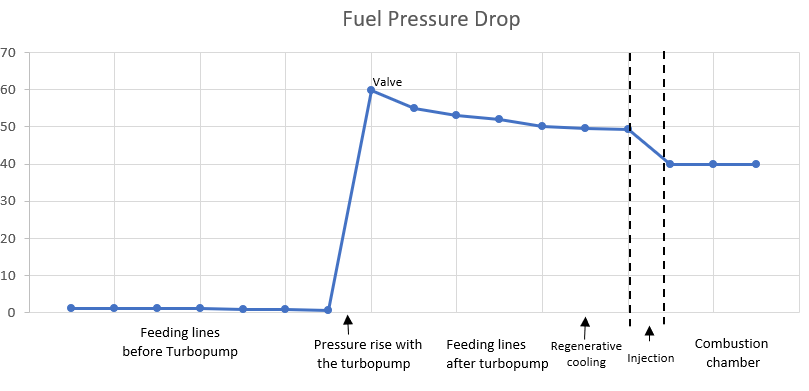
\includegraphics[width=\linewidth]{fuelchart}
	\caption{Pressure evolution on fuel side (bars)}
\end{figure}
\subsection{Oxidizer side}
\begin{table}[H]
	\centering
\begin{tabular}[H]{|c|c|c|}
	\hline
	\cellcolor{gray!50}Contributor& \cellcolor{gray!50}Pressure Drop (bars) & \cellcolor{gray!50}Pressure at the end of this part (bars)\\
	\hline
	Tank & NA & $1.3$ \\
	\hline
	Tank exit & $0.010368$ & $1.29$\\
	\hline
	First section & $0.031$ &$1.259$\\
	\hline
	First bend &$0.25$ &$1.009$\\
	\hline
	Turbo pump & $102.28 $ (Rise) &$108.289$\\
	\hline
	Turbo pump & $5$ &$103.289$\\
	\hline
	Second section &$9.09$ &$94.199$\\
	\hline
	Second bend &$1.06$ &$93.139$\\
	\hline
	Third section &$6.9228$ &$86.2162$\\
	\hline
	Third bend &$1.06$ &$85.1562$\\
	\hline
	Fourth section &$5.366$ &$79.7902$\\
	\hline
	Fourth bend &$1.06$ &$78.7302$\\
	\hline
	Fifth section &$2.7997$ &$75.9305$\\
	\hline
	Catalyzer &$30.95$ &$44.9805$\\
	\hline
	Injection &$4.96$ &$40.0205$\\
	\hline
	Combustion chamber & NA &$40.0205$\\
	\hline
\end{tabular}
\caption{Pressure evolution on fuel side}
\end{table}
\begin{figure}[H]
	\centering
	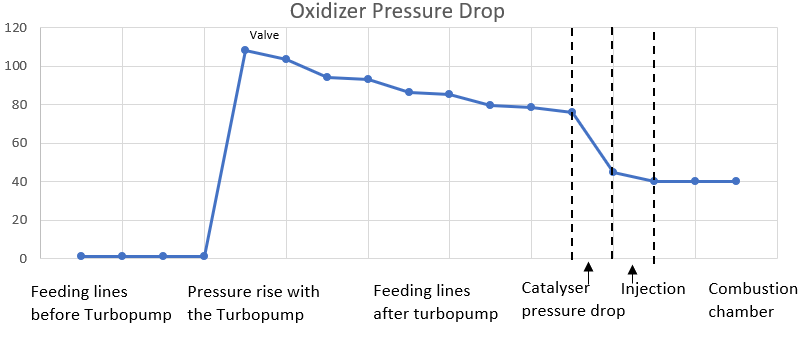
\includegraphics[width=\linewidth]{oxchart}
	\caption{Pressure evolution on oxidizer side (bars)}
\end{figure}
\section{Engine}
\section{Nozzle}
